

%_____________________________________________
\paragraph{Basic facts about the planet}

Facts about planet Mars\footnote{\url{https://en.wikipedia.org/wiki/Mars}}:
\begin{itemize}
\item average radius $R=3389.5 \pm 0.2 \si{\km}$
\item equatorial radius $3396.2 \pm 0.1 \si{\km}$
\item polar radius $3376.2 \pm 0.1 \si{\km}$
\item volume $1.6318 \cdot 10^{20} \si{\cubic\metre}$
\item mass $6.4171 \cdot 10^{23}\si{\kilo\gram}$
\item mean density $\langle\rho\rangle= 3934\si{\kilo\gram\per\cubic\meter}$
\item moment of inertia $I=0.3644 \pm 0.0005$
\item surface gravity $g=3.72076 \si{\metre\per\square\second}$
\end{itemize}

The surface gravity can be obtained with 
\[
g_{surf}=\frac{{\cal G} M}{R^2} 
=\frac{6.67430 \cdot 10^{-11} \; 6.4171 \cdot 10^{23} }{(3.3895\cdot 10^6)^2}
\simeq 3.727977
\]

%_____________________________________________
\paragraph{Internal structure of the planet}

The internal structure of the planet is not settled although 
it is now widely accepted that the planet has a core. News alert: \cite{khcv21,stkb21,knpb21}. 

B. Steinberger was kind enough to communicate to us the density and viscosity 
profiles used in Steinverger \etal (2010) \cite{stwt10} \footnote{Files sent to us 
we slightly altered for the purpose of this work. The density profile was missing 
the 50km near the center of the planet so padding was used. The viscosity profile 
starts below the moho at 50\si{\km} and stopped at the cmb. }:

\begin{center}
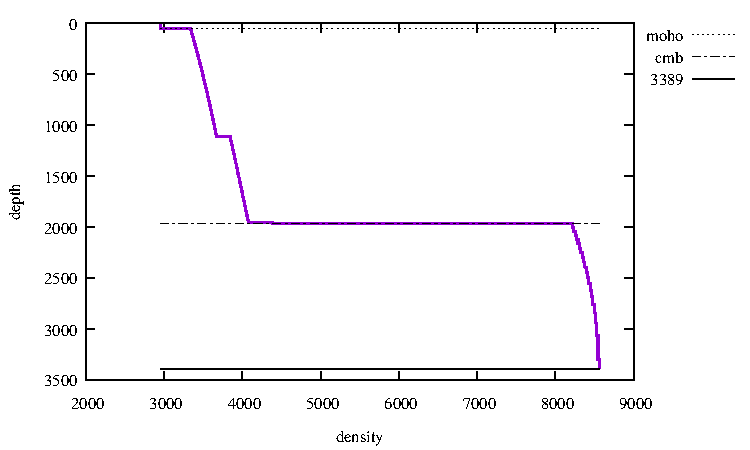
\includegraphics[width=7cm]{python_codes/fieldstone_96/data/rho1}
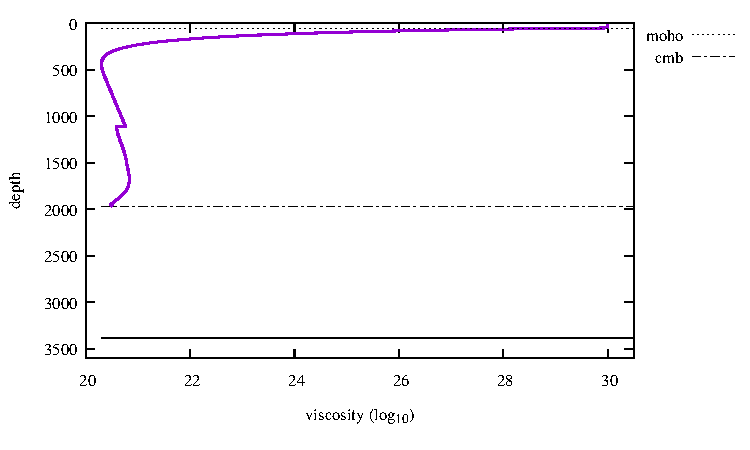
\includegraphics[width=7cm]{python_codes/fieldstone_96/data/eta1}\\
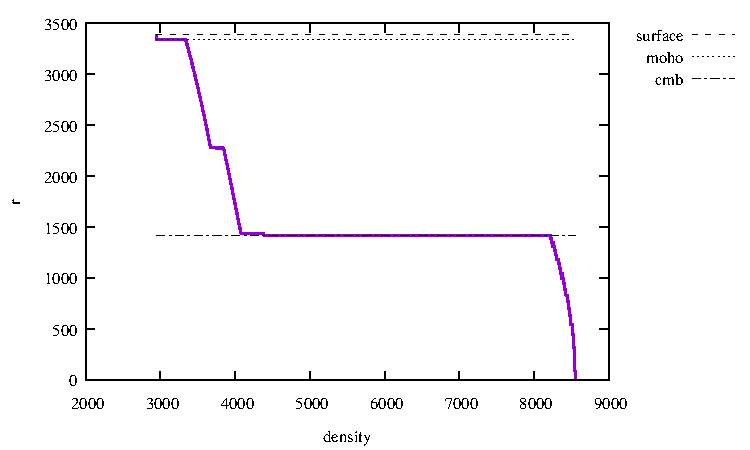
\includegraphics[width=7cm]{python_codes/fieldstone_96/data/rho2}
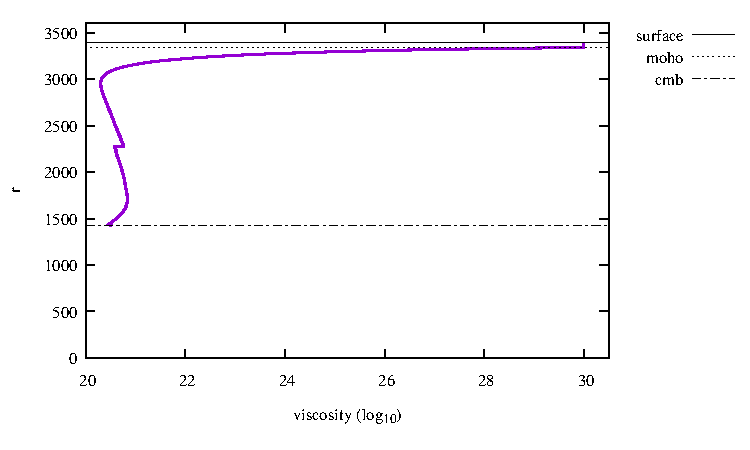
\includegraphics[width=7cm]{python_codes/fieldstone_96/data/eta2}\\
{\captionfont Data curtesy of B. Steinberger, from \cite{stwt10}} \\
{\tiny {\color{gray} in python\_codes/fieldstone\_96/data/}}
\end{center}

\begin{center}
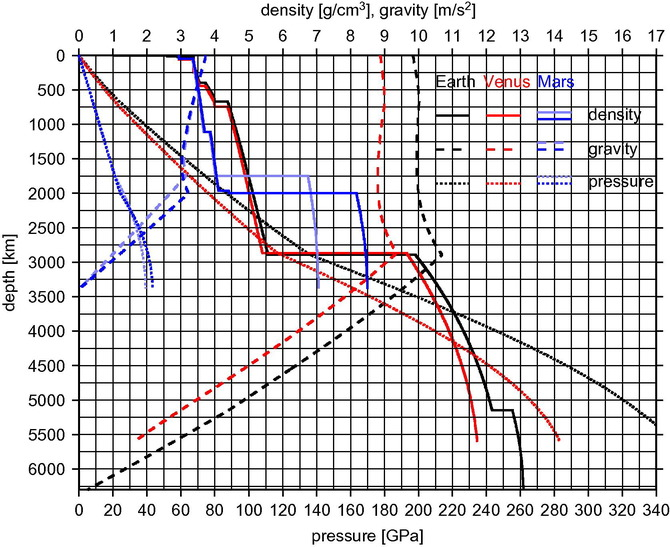
\includegraphics[width=5.7cm]{python_codes/fieldstone_96/images/stwt10_b}
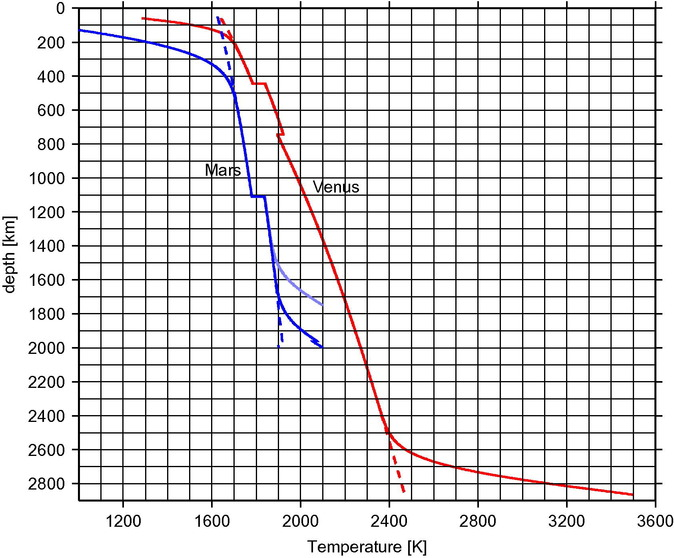
\includegraphics[width=5.7cm]{python_codes/fieldstone_96/images/stwt10_c}
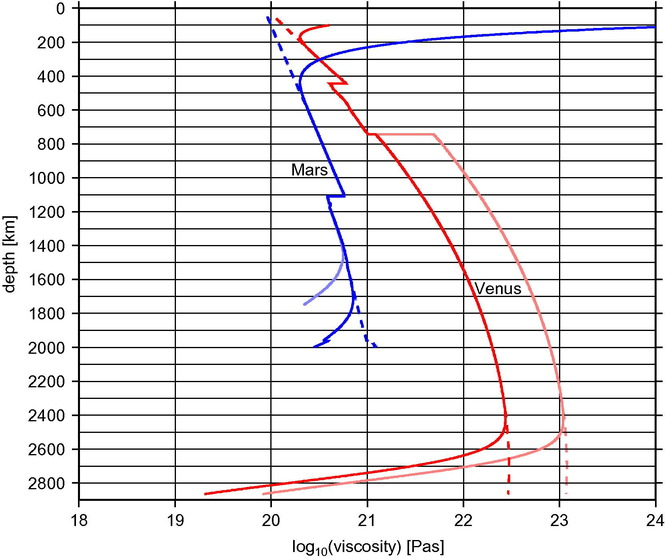
\includegraphics[width=5.7cm]{python_codes/fieldstone_96/images/stwt10_d}\\
{\captionfont Taken from Steinverger \etal (2010) \cite{stwt10}}
\end{center}

In table 1 of Steinberger \etal \cite{stwt10}: crust thickness is set to 50km. The core radius is set 
to 1389.5km. However in the data set we were sent it seems that the cmb is at 1422\si{\km}
radius.
To simplify things we take $R=3389\si{\km}$ and $R_{cmb}=1422\si{\km}$ in the code.

\todo[inline]{Sort this out}

%_______________________________________________________________
\paragraph{How the code works}

There are three python files in this \stone:
\begin{itemize}
\item {\pythonfile parameters.py}: the main physical and geometrical parameters are defined in it;

DESCRIBE PARAMETERS

\item {\pythonfile generate\_nodes.py}: this code generates the two files  {\sl mypoints} and {\sl mysegments}
which will be first concatenated into {\sl mesh.poly} and then passed to the Triangle mesher. 
The mesher then returns {\sl mesh.1.node} and {\sl mesh.1.ele}.  
\item {\pythonfile stone.py} This is the 'real' code: the above mentioned files are read in and are used to 
build the mesh. Density and viscosity profile datasets are read in so that viscosity, density and 
gravity acceleration can then be assigned to elements/nodes/quadrature points. Boundary conditions 
are set up, the FEM is built, and the system solved. The pressure at the surface of the planet is 
normalised to zero average. Results are then exported to ascii and vtu file(s).
\end{itemize}
In order to run the code, simply make use of the provided script {\shellscriptfile run\_script}. 
In it the call to the Triangle mesher is carried out:
\begin{verbatim}
../../../../triangle/triangle   -q -j -O -a5000000000 -o2 -pc  mesh.poly
\end{verbatim}
The number following the {\tt -a} option is the maximum size of an element. This controls the 
average size of the generated elements inside the domain. Decreasing this number automatically 
generates more elements, i.e. a higher resolution. 

The code relies on $P_2\times P_1$ elements or Crouzeix-Raviart elements. Fluids are Newtonian and 
temperature effects are neglected. 

We assume that the problem is axisymmetric, which allows us to simplify the equations greatly. 
We here rely on axisymmetric cylindrical coordinates, see Section~\ref{ss:axicyleqs}.
As shown on the following figure we assume that the deformation/flow is independent of the angle 
$\theta$ so that the remaining space coordinates are $r$ and $z$.
\begin{center}
\begin{flushright} {\tiny {\color{gray} (tikz\_axi.tex)}} \end{flushright}
%~~~~~~~~~~~~~~~~~~~~~~~~~~~~~~~~~~~~~~~~~~~~~~~~~~~~~~~~~~~~~~~~~~~~~~~~~~~~~~~~~~~~~~~~~~~~~~~~~~

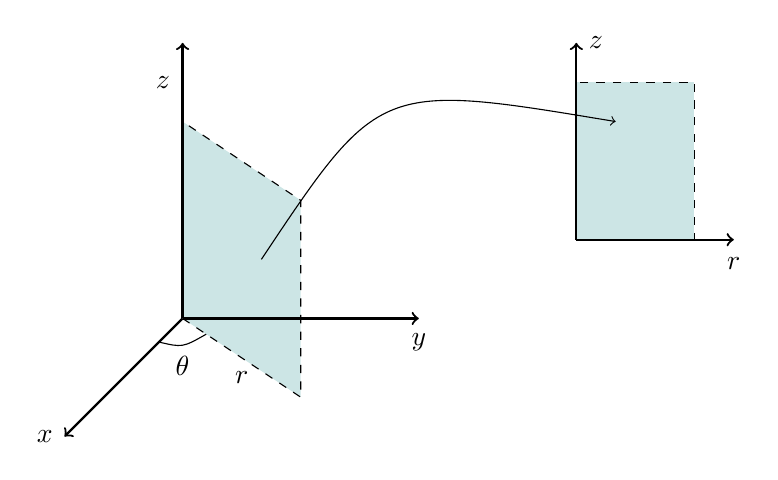
\begin{tikzpicture}
%\draw[step=0.5cm,gray,very thin] (0,0) grid (10,6); %background grid

\draw[dashed,fill=teal!20] (2,2)--(3.5,1)--(3.5,3.5)--(2,4.5)--cycle ;
\draw[thick,->] (2,2) -- (0.5,0.5); 
\draw[thick,->] (2,2) -- (5,2); 
\draw[thick,->] (2,2) -- (2,5.5); 
\node[] at (0.25,0.5) {$x$};
\node[] at (5,1.7) {$y$};
\node[] at (1.75,5) {$z$};
\node[] at (2.75,1.25) {$r$};
\node[] at (2,1.4) {$\theta$};
\draw[] (1.7,1.7) .. controls (2,1.63) ..   (2.3,1.8);

\draw[dashed,fill=teal!20] (7,3)--(8.5,3)--(8.5,5)--(7,5)--cycle; 
\draw[thick,->] (7,3) -- (9,3); 
\draw[thick,->] (7,3) -- (7,5.5); 
\node[] at (9,2.7) {$r$};
\node[] at (7.25,5.5) {$z$};

\draw[->] (3,2.75) .. controls (4.5,5) .. (7.5,4.5);
\end{tikzpicture}



\end{center}

%\begin{center}
%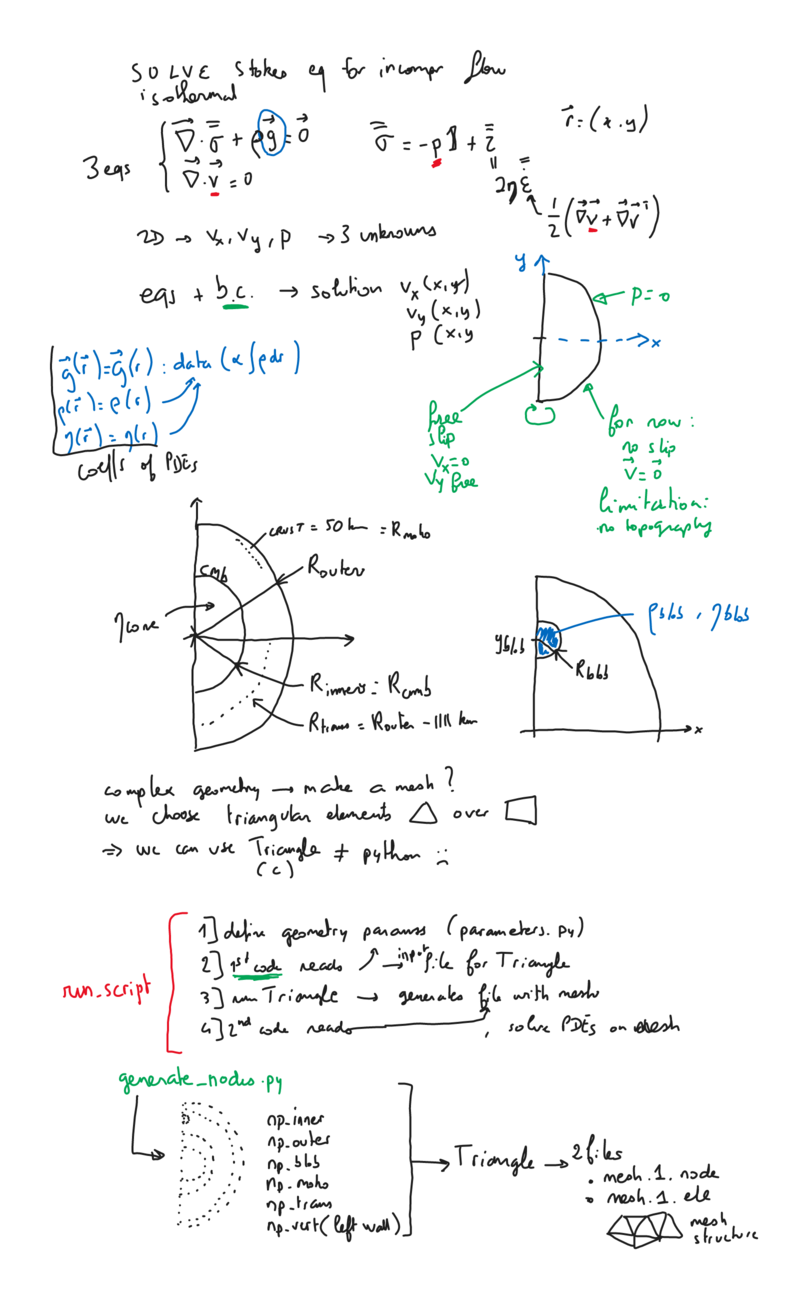
\includegraphics[width=7cm]{python_codes/fieldstone_96/images/notes1}\\
%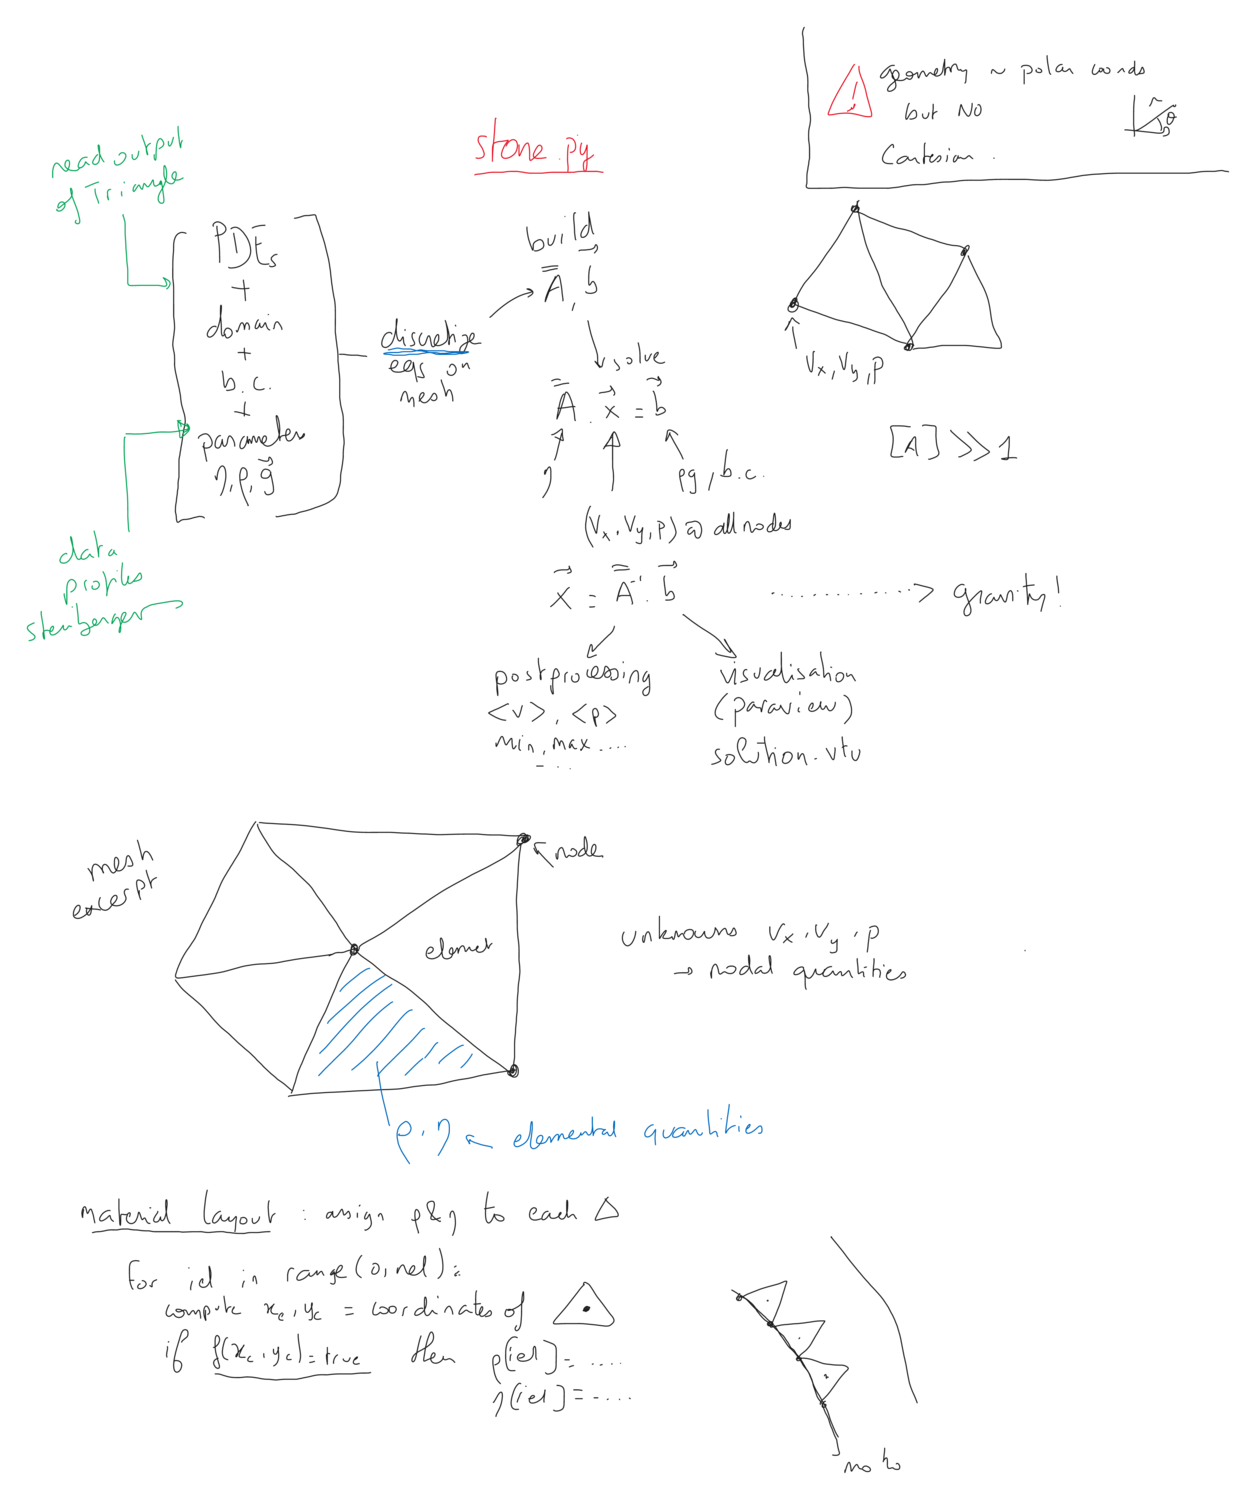
\includegraphics[width=9cm]{python_codes/fieldstone_96/images/notes2}
%\end{center}

We assume here that the fluid is incompressible.
Given the symmetry of the problem any term containing $\partial_\theta$ or $\upnu_\theta$ is zero.
The strain rate tensor given in Section~\ref{ss:srcc} then simplifies to:

\begin{eqnarray}
\dot\varepsilon_{rr} 
&=& \frac{\partial \upnu_r}{\partial r} \nn\\
\dot\varepsilon_{\theta\theta}  &=& \frac{\upnu_r}{r} \nn\\
\dot\varepsilon_{\theta r} = \dot\varepsilon_{r\theta}  &=& 0 \nn\\
\dot\varepsilon_{zz} &=& \frac{\partial \upnu_z}{\partial z} \nn\\
\dot{\varepsilon}_{rz} = \dot{\varepsilon}_{zr} 
&=& \frac{1}{2}\left( \frac{\partial \upnu_r}{\partial z} + \frac{\partial \upnu_z}{\partial r} \right) \nn\\
\dot{\varepsilon}_{\theta z} = \dot{\varepsilon}_{z \theta} &=& 0 \nn
\end{eqnarray}
Note that the term $\dot\varepsilon_{\theta\theta} $ is not zero!
The deviatoric stress tensor ${\bm \tau}=2\eta \dot{\bm \varepsilon}$ can be computed
as well as the full stress tensor ${\bm \sigma}=-p {\bm 1} + {\bm \tau}$. 

%\begin{center}
%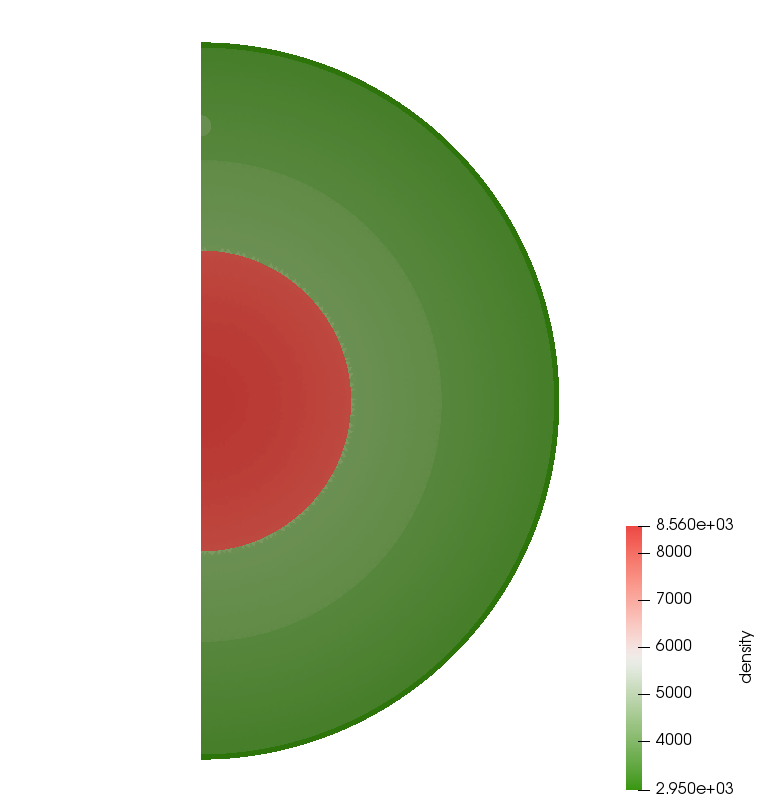
\includegraphics[width=6cm]{python_codes/fieldstone_96/images/rho}
%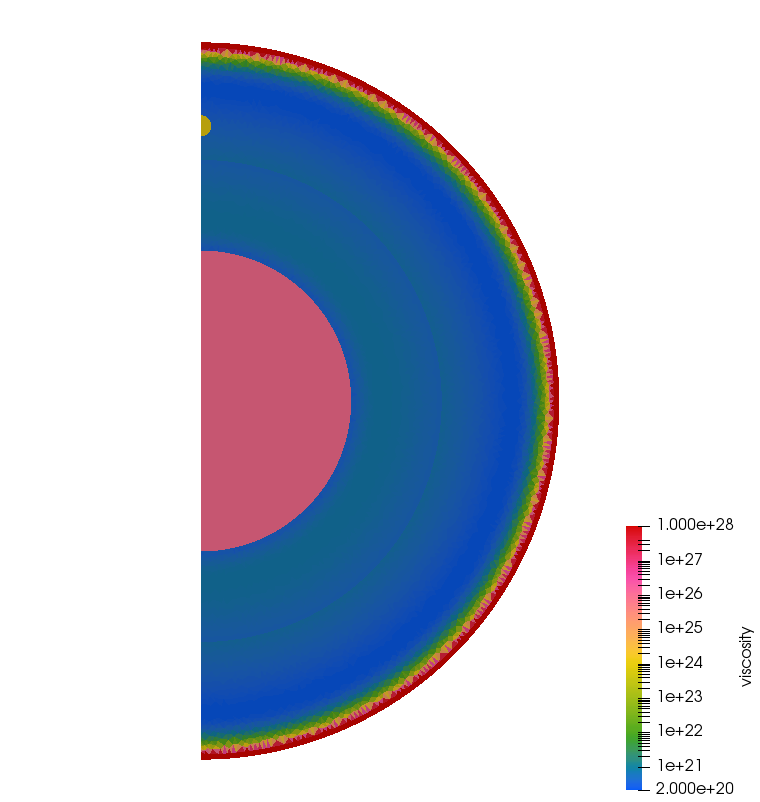
\includegraphics[width=6cm]{python_codes/fieldstone_96/images/eta}
%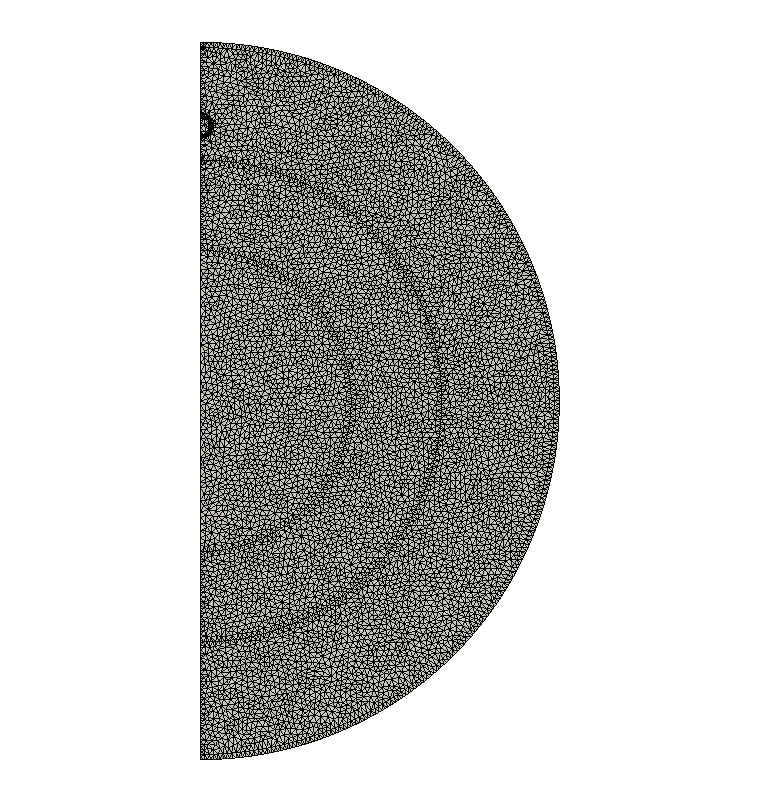
\includegraphics[width=6cm]{python_codes/fieldstone_96/images/mesh}
%\end{center}

ONE problem remains: I have not yet found out how to remove the core altogether!
so for now I set zero velocity at cmb nodes (equivalent to no slip).

%__________________________________________________________________
\paragraph{About pressure normalisation}

We actually want to compute 
\[
\langle p \rangle _\Gamma = \frac{1}{4\pi R_o^2} \iiint \delta(r-R_o) p(\theta) r^2 \sin\theta \; dr d\theta d\phi 
= \frac{1}{2} \int_0^\pi p(\theta) \sin\theta \; d\theta
\]
The integral is then carried out by finding the elements for which two vertices are on the outside boundary, 
computing the angular opening $d\theta$, the average pressure along the edge and the value of $\sin\theta$ at the
middle of the edge. 
The obtained value is then subtracted from the pressure. 

%__________________________________________________________________
\paragraph{From Cylindrical to Cartesian coordinates}

In cylindrical coordinates, and in the axisymmetric case
the strain rate tensor is given by
\[
\dot{\bm\varepsilon}(\vec\upnu)
=
\left(
\begin{array}{ccc}
\dot\varepsilon_{rr} & 0 & \dot{\varepsilon}_{rz} \\
0 & \dot{\varepsilon}_{\theta\theta}  & 0 \\
\dot{\varepsilon}_{zr} & 0 & \dot\varepsilon_{zz}
\end{array}
\right)
\]
We will now convert it to Cartesian coordinates using the equation from \url{https://www.brown.edu/Departments/Engineering/Courses/En221/Notes/Polar_Coords/Polar_Coords.htm}, where ${\bm T}$ is a tensor:
\[
{\bm T}_{\tiny Cyl}=
\left(
\begin{array}{ccc}
T_{rr}       & T_{r\theta}      & T_{rz} \\
T_{\theta r} & T_{\theta\theta} & T_{\theta z} \\
T_{z r}      & T_{z \theta}     & T_{zz}
\end{array}
\right)
=
\left(
\begin{array}{ccc}
 \cos \theta&\sin \theta&0 \\
-\sin \theta&\cos \theta&0 \\
0 & 0 & 1 
\end{array}
\right)
\cdot
\left(
\begin{array}{ccc}
T_{xx} & T_{xy} & T_{xz} \\
T_{yx} & T_{yy} & T_{yz} \\
T_{zx} & T_{zy} & T_{zz} 
\end{array}
\right)
\cdot
\left(
\begin{array}{ccc}
\cos \theta & -\sin \theta&0 \\
\sin \theta &  \cos \theta&0 \\
0 & 0 & 1 
\end{array}
\right)
\]

\[
{\bm T}_{\tiny Cart}=
\left(
\begin{array}{ccc}
T_{xx} & T_{xy} & T_{xz} \\
T_{yx} & T_{yy} & T_{yz} \\
T_{zx} & T_{zy} & T_{zz} 
\end{array}
\right)
=
\left(
\begin{array}{ccc}
 \cos \theta&-\sin \theta&0 \\
\sin \theta&\cos \theta&0 \\
0 & 0 & 1 
\end{array}
\right)
\cdot
\left(
\begin{array}{ccc}
T_{rr}       & T_{r\theta}      & T_{rz} \\
T_{\theta r} & T_{\theta\theta} & T_{\theta z} \\
T_{z r}      & T_{z \theta}     & T_{zz}
\end{array}
\right)
\cdot
\left(
\begin{array}{ccc}
\cos \theta & \sin \theta&0 \\
-\sin \theta &  \cos \theta&0 \\
0 & 0 & 1 
\end{array}
\right)
\]
In our case the calculation is taking place in the $(x,z)$
plane, i.e. $\theta=0$ so that the rotation matrices above 
are in fact identity matrices. 
We then simply have 
$\dot{\bm \varepsilon}_{\tiny Cart}=
\dot{\bm \varepsilon}_{\tiny Cyl}$.


%__________________________________________________________________
\paragraph{From Cartesian to Spherical coordinates}

We have
\begin{eqnarray}
{\bm T}_{\tiny Sph}&=&
\left(
\begin{array}{ccc}
T_{rr}       & T_{r\theta}      & T_{r\phi} \\
T_{\theta r} & T_{\theta\theta} & T_{\theta\phi} \\
T_{\phi r}   & T_{\phi \theta}  & T_{\phi\phi}
\end{array}
\right) \nn\\
&=&
\left(
\begin{array}{ccc}
\sin\theta \cos\phi & \sin\theta \sin\phi & \cos\theta \\
\cos\theta \cos\phi & \cos\theta \sin\phi & -\sin\theta \\
-\sin\phi & \cos\phi & 0 
\end{array}
\right)
\cdot
\left(
\begin{array}{ccc}
T_{xx} & T_{xy} & T_{xz} \\
T_{yx} & T_{yy} & T_{yz} \\
T_{zx} & T_{zy} & T_{zz} 
\end{array}
\right)
\cdot
\left(
\begin{array}{ccc}
\sin\theta\cos\phi & \cos\theta\cos\phi & -\sin\phi \\
\sin\theta\sin\phi & \cos\theta\sin\phi & \cos\phi \\
\cos\theta & -\sin\theta & 0
\end{array}
\right) 
\nn\\
{\bm T}_{\tiny Cart} &=&
\left(
\begin{array}{ccc}
T_{xx} & T_{xy} & T_{xz} \\
T_{yx} & T_{yy} & T_{yz} \\
T_{zx} & T_{zy} & T_{zz} 
\end{array}
\right) \nn\\
&=&
\left(
\begin{array}{ccc}
\sin\theta\cos\phi & \cos\theta\cos\phi & -\sin\phi \\
\sin\theta\sin\phi & \cos\theta\sin\phi & \cos\phi \\
\cos\theta & -\sin\theta & 0
\end{array}
\right)
\cdot
\left(
\begin{array}{ccc}
T_{rr}       & T_{r\theta}      & T_{r\phi} \\
T_{\theta r} & T_{\theta\theta} & T_{\theta\phi} \\
T_{\phi r}   & T_{\phi \theta}  & T_{\phi\phi}
\end{array}
\right)
\cdot
\left(
\begin{array}{ccc}
\sin\theta \cos\phi & \sin\theta \sin\phi & \cos\theta \\
\cos\theta \cos\phi & \cos\theta \sin\phi & -\sin\theta \\
-\sin\phi & \cos\phi & 0 
\end{array}
\right)
\end{eqnarray}
In our case, calculations take place in the 
$(x,z)$-plane so we have $\phi=0$ and the equation above 
becomes
\[
\left(
\begin{array}{ccc}
T_{rr}       & T_{r\theta}      & T_{r\phi} \\
T_{\theta r} & T_{\theta\theta} & T_{\theta\phi} \\
T_{\phi r}   & T_{\phi \theta}  & T_{\phi\phi}
\end{array}
\right)
=
\left(
\begin{array}{ccc}
\sin\theta  & 0 & \cos\theta \\
\cos\theta  & 0 & -\sin\theta \\
0 & 1 & 0 
\end{array}
\right)
\cdot
\left(
\begin{array}{ccc}
T_{xx} & T_{xy} & T_{xz} \\
T_{yx} & T_{yy} & T_{yz} \\
T_{zx} & T_{zy} & T_{zz} 
\end{array}
\right)
\cdot
\left(
\begin{array}{ccc}
\sin\theta & \cos\theta & 0 \\
0 & 0 & 1 \\
\cos\theta & -\sin\theta & 0
\end{array}
\right)
\]
We define $c_\theta=\cos\theta$, $s_\theta=\sin\theta$ so that
\[
\left(
\begin{array}{ccc}
T_{rr}       & T_{r\theta}      & T_{r\phi} \\
T_{\theta r} & T_{\theta\theta} & T_{\theta\phi} \\
T_{\phi r}   & T_{\phi \theta}  & T_{\phi\phi}
\end{array}
\right)
=
\left(
\begin{array}{ccc}
s_\theta  & 0 & c_\theta \\
c_\theta  & 0 & -s_\theta \\
0 & 1 & 0 
\end{array}
\right)
\cdot
\left(
\begin{array}{ccc}
T_{xx} & T_{xy} & T_{xz} \\
T_{yx} & T_{yy} & T_{yz} \\
T_{zx} & T_{zy} & T_{zz} 
\end{array}
\right)
\cdot
\left(
\begin{array}{ccc}
s_\theta & c_\theta & 0 \\
0 & 0 & 1 \\
c_\theta & -s_\theta & 0
\end{array}
\right)
\]
As we have seen above we have 
\[
\dot{\bm\varepsilon}_{\tiny Cart}
=
\left(
\begin{array}{ccc}
\dot\varepsilon_{xx} & 0 & \dot{\varepsilon}_{xz} \\
0 & \dot{\varepsilon}_{yy}  & 0 \\
\dot{\varepsilon}_{xz} & 0 & \dot\varepsilon_{zz}
\end{array}
\right)
\]
so 
\begin{eqnarray}
\dot{\bm \varepsilon}_{\tiny Sph}=
\left(
\begin{array}{ccc}
\dot\varepsilon_{rr}       & \dot\varepsilon_{r\theta}      & \dot\varepsilon_{r\phi} \\
\dot\varepsilon_{\theta r} & \dot\varepsilon_{\theta\theta} & \dot\varepsilon_{\theta\phi} \\
\dot\varepsilon_{\phi r}   & \dot\varepsilon_{\phi \theta}  & \dot\varepsilon_{\phi\phi}
\end{array}
\right)
&=&
\left(
\begin{array}{ccc}
s_\theta  & 0 & c_\theta \\
c_\theta  & 0 & -s_\theta \\
0 & 1 & 0 
\end{array}
\right)
\cdot
\left(
\begin{array}{ccc}
\dot\varepsilon_{xx} & 0 & \dot{\varepsilon}_{xz} \\
0 & \dot{\varepsilon}_{yy}  & 0 \\
\dot{\varepsilon}_{xz} & 0 & \dot\varepsilon_{zz}
\end{array}
\right)
\cdot
\left(
\begin{array}{ccc}
s_\theta & c_\theta & 0 \\
0 & 0 & 1 \\
c_\theta & -s_\theta & 0
\end{array}
\right)  \nonumber\\
&=&
\left(
\begin{array}{ccc}
s_\theta  & 0 & c_\theta \\
c_\theta  & 0 & -s_\theta \\
0 & 1 & 0 
\end{array}
\right)
\cdot
\left(
\begin{array}{ccc}
\dot\varepsilon_{xx} s_\theta + 
\dot\varepsilon_{xz} c_\theta  & 
\dot\varepsilon_{xx} c_\theta - 
\dot\varepsilon_{xz} s_\theta  &
0 \\
0 & 0 & \dot{\varepsilon}_{yy}  
\\
\dot\varepsilon_{xz} s_\theta + 
\dot\varepsilon_{zz} c_\theta  &
\dot\varepsilon_{xz} c_\theta - 
\dot\varepsilon_{zz} s_\theta  &
0 
\end{array}
\right)  \nonumber\\
&=&
\left(
\begin{array}{ccc}
\dot\varepsilon_{xx} s_\theta^2 + 
2 \dot\varepsilon_{xz} c_\theta  s_\theta +
\dot\varepsilon_{zz} c_\theta ^2  
& 
\dot\varepsilon_{xx} c_\theta s_\theta - 
\dot\varepsilon_{xz} s_\theta^2  +
\dot\varepsilon_{xz} c_\theta^2 - 
\dot\varepsilon_{zz} s_\theta c_\theta 
& 0 \\ \\
\dot\varepsilon_{xx} s_\theta c_\theta+ 
\dot\varepsilon_{xz} c_\theta^2  -
\dot\varepsilon_{xz} s_\theta^2 -
\dot\varepsilon_{zz} c_\theta s_\theta 
&
\dot\varepsilon_{xx} c_\theta^2 - 
2\dot\varepsilon_{xz} s_\theta c_\theta +
\dot\varepsilon_{zz} s_\theta^2  
& 0 
\\ \\
0 & 0 & \dot{\varepsilon}_{yy} 
\end{array}
\right)  \nonumber
\end{eqnarray}
We can easily verify that the trace of this tensor is zero.

The deviatoric stress is given by 
${\bm \tau}=2\eta \dot{\bm \varepsilon}$,
the traction at the surface  by 
$\vec{t}={\bm \tau}\cdot \vec{n}$ (
with $\vec{n}=\vec{e}_r$ at the surface in Spherical coordinates) and the normal to the surface component of this traction 
is given by
\[
t_r = \vec{t}\cdot \vec{n} = ({\bm \tau}\cdot \vec{n})\cdot \vec{n} = \tau_{rr}
\]


%_____________________________________________________________
\paragraph{A proxy for elasto-viscous lithospheric rheology}

The implementation of elastic behaviour in a velocity-pressure code is not trivial and is presented in Section~\ref{ss:evrheo}.
In the end the lithospheric viscosity will be an effective viscosity given by
\[
\eta_{eff} = \frac{\mu \delta t}{1+\mu/\eta \delta t} 
\]
This is only used if \texttt{use\_ev} is true.


%_____________________________________________________________
\paragraph{Comparing with \aspect}

We define a simple geometry: there are 3 materials in the domain: the `crust' between 0 and 100km depth, 
the `lithosphere' between 100 and 500km depth and the mantle down to the cmb at 1600km depth.
Based on Steinberger \etal \cite{stwt10}, we take $\eta_{mantle}=6\cdot 10^{20}$, and $\eta_{lith}=10^{21}$
while the crust viscosity will be varied over several orders of magnitude.
For simplicity we take the gravitational to be constant in the model at $g=3.72$.

The blob has a radius of 300km and its center is located 1000km below the north pole of the planet.
It is therefore entirely in the mantle and its relative density with regards to the mantle is $\delta\rho=-200$.

 
%--------------------------------------------------
\subsubsection*{Gravity calculations}

This is an axisymmetric problem so the mesh is generated for a single value of the cylindrical 
coordinates $\theta$ angle. 
This makes gravity calculations a bit more difficult because each triangle of the mesh corresponds
in 3D to a ring of matter with this triangular cross section. 
I have therefore chosen to chunk this ring in {\tt nel\_phi} bits. Each bit has a given volume and therefore
mass, and having computed its center its generated gravity field can be added. 
The volume of such a block is $\iiint_{block} r dr d\theta dz =\iint_\triangle rdrdz \cdot \int d\theta$.  
The first integral is carried out for each triangle and the result is stored in the {\tt arear} array. 

NOT FINISHED/TESTED

Look at Morgan (1965) \cite{morg65} for gravity anomalies above sinking sphere. 




